\documentclass[12pt]{article}
\usepackage[T1]{fontenc}
\usepackage[utf8]{inputenc}
\usepackage[polish]{babel}

\usepackage{alltt}
\usepackage{varioref}
\usepackage{enumerate}
\usepackage{amsfonts}
\usepackage{amsmath} 
\usepackage{indentfirst}
\usepackage{graphicx} 
\usepackage{float}
\usepackage{subfig}
\usepackage{listings} 
\usepackage{multirow}
\usepackage{pdfpages}
\usepackage[usenames,dvipsnames,table]{xcolor}
%\usepackage[hdivide={2cm,*,2cm},vdivide={2cm,*,2.5cm}]{geometry}
\frenchspacing

\makeatletter
\def\namedlabel#1#2{\begingroup
   \def\@currentlabel{#2}%
   \label{#1}\endgroup
}
\makeatother
\linespread{1.3}
\usepackage[a4paper, left=2.5cm, right=2.5cm, top=2.5cm, bottom=2.5cm, headsep=1.2cm]{geometry}

% kolory
\usepackage[usenames,dvipsnames]{xcolor}
%Apricot 	Aquamarine 	Bittersweet 	Black
%Blue		BlueGreen 	BlueViolet 	BrickRed
%Brown 		BurntOrange 	CadetBlue 	CarnationPink
%Cerulean 	CornflowerBlue 	Cyan	 	Dandelion
%DarkOrchid 	Emerald 	ForestGreen 	Fuchsia
%Goldenrod 	Gray	 	Green	 	GreenYellow
%JungleGreen 	Lavender 	LimeGreen 	Magenta
%Mahogany 	Maroon	 	Melon	 	MidnightBlue
%Mulberry 	NavyBlue 	OliveGreen 	Orange
%OrangeRed 	Orchid	 	Peach	 	Periwinkle
%PineGreen 	Plum	 	ProcessBlue 	Purple
%RawSienna 	Red	 	RedOrange 	RedViolet
%Rhodamine 	RoyalBlue 	RoyalPurple 	RubineRed
%Salmon 	SeaGreen 	Sepia	 	SkyBlue
%SpringGreen 	Tan	 	TealBlue 	Thistle
%Turquoise 	Violet	 	VioletRed 	White
%WildStrawberry Yellow	 	YellowGreen 	YellowOrange

\usepackage{hyperref} % musi być ostatni!!
\hypersetup{
    bookmarks=true,         % show bookmarks bar?
    pdftoolbar=true,        % show Acrobat's toolbar?
    pdfmenubar=true,        % show Acrobat's menu?
    pdffitwindow=false,     % window fit to page when opened
    pdfstartview={FitH},    % fits the width of the page to the window
    pdfnewwindow=true,      % links in new window
    colorlinks=true,        % false: boxed links; true: colored links
    linkcolor=Black,%MidnightBlue,    % color of internal links
    citecolor=Black,%Plum,        % color of links to bibliography
    filecolor=Black,%magenta,      % color of file links
    urlcolor=Black%cyan           % color of external links
}
%%%%%%%%%%%%%%%%%%%%%%%%%%%%%%%%%%%%%%%%%%%%%%%%%%%%%%%%%%%%%%%%%%%%%%%%%%%%%%%%%%%%%%%%%%%%%%%%%%%%%%%%%%%%%%%%%%%%%%%%%%%%%%%%%%
% początek dokumentu
\begin{document}
\graphicspath{{obrazki}}
\begin{titlepage}
\vspace*{\fill}
 \begin{center}

  \textsc{\LARGE Systemy inteligentnych agentów}\\[2.0cm]
  \textsc{\Large Symulacja rynku spożywczego}\\[1.5cm] 

\vspace*{\fill}
% autorzy:
  \begin{minipage}{0.4\textwidth}
    \begin{flushleft} \large
    \emph{Autorki:}\\
    Weronika Świderska, 233221 \\ Beata Wójciak, 241772
    \end{flushleft}
    \end{minipage}
    \begin{minipage}{0.4\textwidth}
    \begin{flushright} \large
    \emph{Prowadzący:} \\
    Piotr Lipiński
    \end{flushright}
  \end{minipage}

%\vfill
\vspace*{\fill}
% Bottom of the page
{\large \today}
 \end{center}

\end{titlepage}
\newpage
%spis treści
\tableofcontents
\newpage

\section{Wprowadzenie}
Celem naszego projektu było stworzenie systemu inteligentnych agentów, które~---~dzięki wzajemnej komunikacji~---~miały symulować działanie rynku spożywczego.

W~projekcie uwzględniłyśmy kilka różnych typów agentów różniących się zarówno rolami jak i~strategiami.

\section{Opis projektu}
Na naszym rynku działało 6~różnych typów agentów na 3~różnych poziomach:
\begin{itemize}\label{items:typy agentów}
 \item Poziom~1: agenci, którzy produkują najbardziej podstawowe towary, należą tu:
  \begin{itemize}
  \item Rolnik (produkuje zboże, \verb GRAIN )~---~\verb FARMER .
  \item Hodowca (produkuje mięso~---~\verb MEAT , mleko~---~\verb MILK  i~nawóz~---~\verb MANURE )~---~\verb KEEPER .
  \item Sadownik (produkuje owoce, \verb FRUIT )~---~\verb GROWER .
  \end{itemize}
 \item Poziom~2: agenci, którzy kupują towary od agentów 1~poziomu, przetwarzają je, a~następnie sprzedają dalej. Należą tu:
  \begin{itemize}
   \item Piekarz (kupuje zboże, a~sprzedaje pieczywo~---~\verb BREAD )~---~\verb BAKER .
   \item Mleczarz (kupuje mleko, a~sprzedaje produkty mleczne~---~\verb MILK_PRODUCT )~---~\verb MILKMAN .
  \end{itemize}
 \item Poziom~3: należą tu tylko agenci pełniący rolę klientów, którzy nie produkują żadnych dóbr, a~jedynie kupują je od innych~---~\verb CLIENT .
\end{itemize}

Zależności między agentami przedstawia Rysunek \ref{fig:schemat zależności}.
\begin{figure} [H]
 \centering
 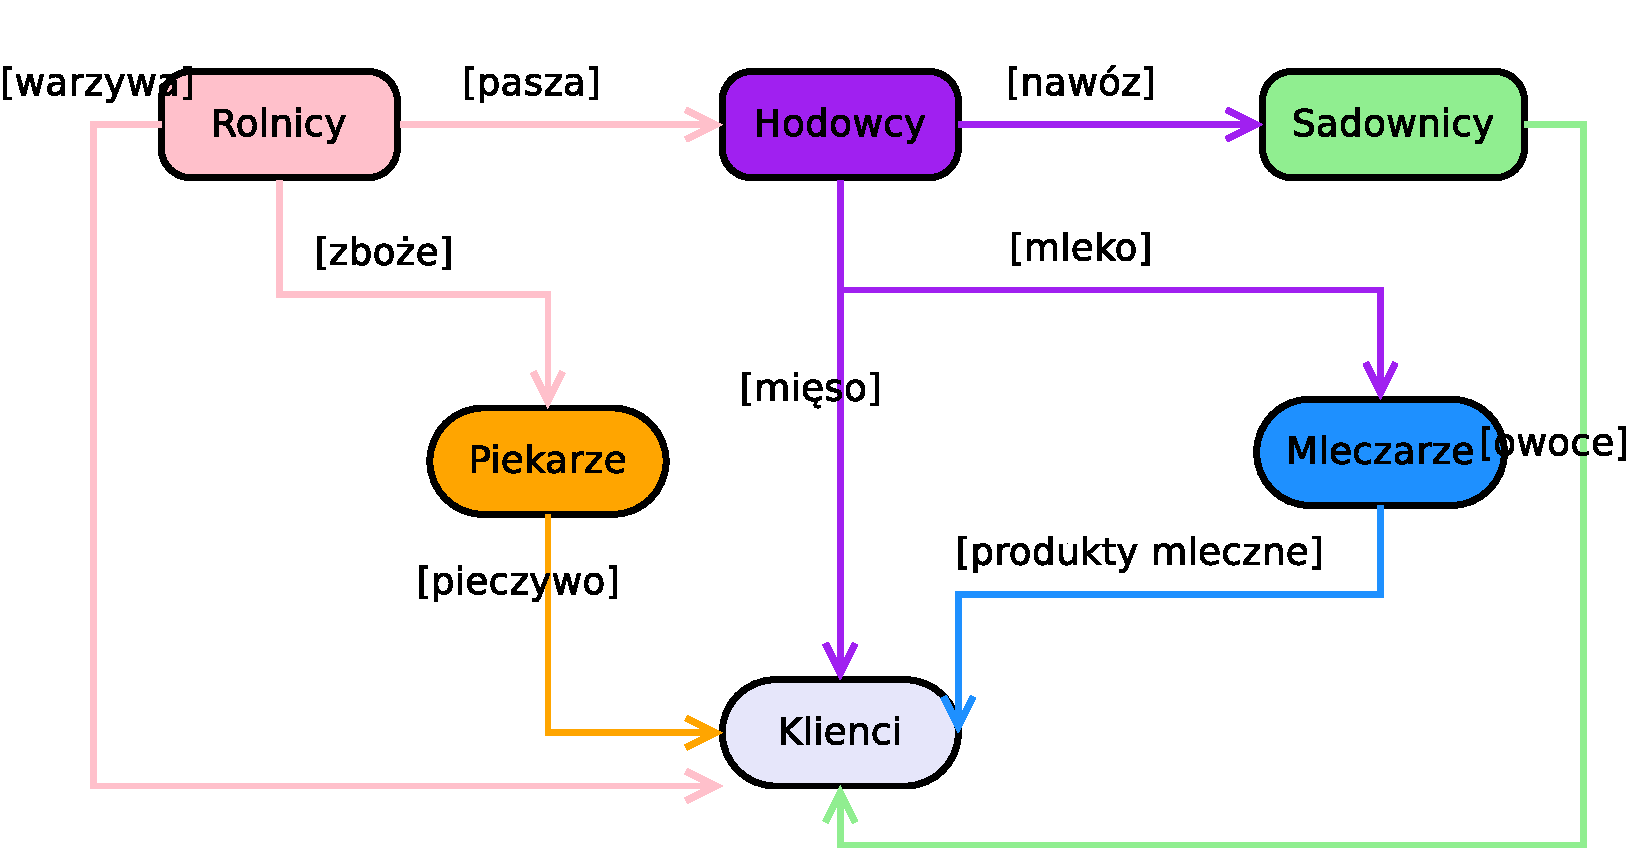
\includegraphics[width=0.8\textwidth]{obrazki/diagram_kolorowy}
 \caption{Schemat zależności między agentami}
 \label{fig:schemat zależności}
\end{figure}

Na początku każdy agent dostaje pewną ilość dóbr, które może zużyć na handel lub wytworzenie większej ilości produktów (np. obsiać pole). Wielkość początkowych zasobów agenta ma wpływ na to, jak radzi on sobie
na rynku~---~szczegółowe wyniki z tym związane przedstawione zostały w Rozdziale~\ref{chapter: rezultaty}.

\section{Architektura systemu}
Program został napisany w~Javie z~wykorzystaniem platformy JADE. Ułatwiło to znacznie implementację komunikacji między agentami zgodnie ze standardami FIPA.

W~celu utworzenia statystyk działania agentów wszelkie informacje zapisywane są do plików przy pomocy Apache POI, na podstawie których tworzone są następnie wykresy obrazujące zasoby poszczególnych agentów w~zależności od czasu.

\section{Komunikacja między agentami}
\subsection{Etapy komunikacji}
Komunikacja między agentami odbywa się w~kilku etapach. W~każdym etapie muszą być przeprowadzone pewne akcje, które następnie są komunikowane drugiej stronie.

Podczas dokonywania transakcji
można wyróżnić następujące etapy (schemat komunikacji przedstawia Rysunek~\ref{fig:schemat komunikacji}, stworzony przy pomocy narzędzia \emph{Sniffer} będącego częścią platformy JADE):
\begin{enumerate}
 \item Na początku każdego tygodnia każdy agent, który sprzedaje jakiś produkt informuje potencjalnych kupców co sprzedaje, w~jakiej cenie i~w~jakiej ilości. Wysyła to za pomocą komunikatu typu \verb INFORM  (czarna strzałka
na Rysunku \ref{fig:schemat komunikacji}).
 \item Po otrzymaniu ofert od wszystkich sprzedających oferujących dobro poszukiwane przez kupca, podejmuje on decyzję, na które oferty się może przystać i~na jakich warunkach (może zaoferować inną cenę i~ilość niż sprzedający).
 \item Kupujący odsyła sprzedającemu swoje propozycje (lub pustą wiadomość, by dać znać, że nie jest zainteresowany daną ofertą) używając komunikatu typu \verb CFP  (górna szara strzałka
na Rysunku \ref{fig:schemat komunikacji}).
 \item Po otrzymaniu propozycji od wszystkich kupujących, do których sprzedający wysłał wiadomość sprzedający analizuje oferty i~podejmuje ostateczną decyzję co do tego, na jakie transakcje przystaje. 
Wysyła klientom swoje decyzje korzystając z~komunikatu typu \verb PROPOSE  (górna błękitna strzałka
na Rysunku \ref{fig:schemat komunikacji}).
 \item Klient po otrzymaniu i~analizie decyzji od sprzedającego akceptuje ją lub odrzuca, o~czym informuje sprzedającego komunikatem typu \verb ACCEPT_PROPOSAL \newline albo \verb REJECT_PROPOSAL  (dolna szara strzałka
na Rysunku \ref{fig:schemat komunikacji}).
 \item Jeśli sprzedawca otrzymał zgodę kupującego na transakcję, to sprawdza, czy może ona wciąż być zrealizowana (czy w~międzyczasie towary nie zostały sprzedane komuś innemu).
Jeśli wszystko jest w~porządku potwierdza klientowi wykonanie transakcji komunikatem typu \verb CONFIRM  i~aktualizuje stan posiadanych produktów. W~przeciwnym razie wysyła komunikat typu \verb REFUSE  (dolna błękitna strzałka
na Rysunku \ref{fig:schemat komunikacji}).
 \item Po otrzymaniu potwierdzenia wykonania transakcji kupujący również uaktualnia zawartość swoich magazynów.
\end{enumerate}

\begin{figure} [H]
 \centering
 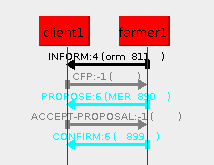
\includegraphics[width=0.7\textwidth]{obrazki/komunikacja_2_agentow-accept}
 \caption{Schemat komunikacji między przykładowymi agentami}
 \label{fig:schemat komunikacji}
\end{figure}

Przykładowa transakcja z~wykorzystaniem większej liczby agentów przedstawiona jest na Rysunku \ref{fig:sytuacje w komunikacji}. 

\begin{figure} [H]
 \centering
    \subfloat{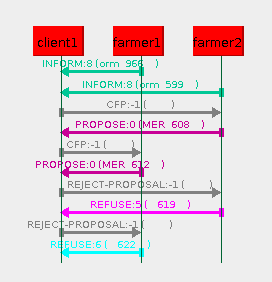
\includegraphics[width=0.45\textwidth]{obrazki/komunikacja_3_agentow-refuse} \label{fig: odrzuć oba}}\hspace{20pt}
    \subfloat{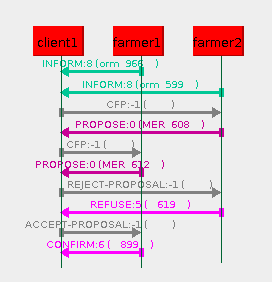
\includegraphics[width=0.45\textwidth]{obrazki/komunikacja_3_agentow-refuse_and_accept}\label{fig: zaakceptuj jedno}}\hspace{20pt}
 \caption{Różne możliwe sytuacje podczas transakcji}
 \label{fig:sytuacje w komunikacji}
\end{figure}

Rysunek \ref{fig: odrzuć oba} obrazuje sytuację, w~której agent \emph{client1} nie jest zainteresowany ofertą żadnego z~agentów. 

W~tym wypadku po otrzymaniu ofert od sprzedających i~analizie sytuacji odrzuca obie propozycje sprzedaży,
co oświadcza komunikatem \verb REJECT_PROPOSAL . Otrzymanie informacji potwierdza zarówno \emph{farmer1} jak i~\emph{farmer2} wysyłając wiadomość \verb REFUSE .


Rysunek \ref{fig: zaakceptuj jedno} przedstawia podobną sytuację, jednak w~tym wypadku \emph{client1} zgadza się na ofertę agenta \emph{farmer1}. 

Wysyła mu zatem komunikat \verb ACCEPT_PROPOSAL , na co \emph{farmer1} odpowiada
wiadomością \verb CONFIRM . Gdyby \emph{farmer1} nie był w~stanie dokonać tej transakcji wysłałby komunikat \verb REFUSE .

\subsection{Format oferty}
Komunikaty zawierające ofertę wysyłane przez agentów mają poniższy format:
\begin{itemize}
 \item \verb!FARMER;sell;VEGETABLE 2014.9341514088535 2.0:GRAIN 5171.979684030067 2.0:!
 \item \verb!BAKER;buy;GRAIN 140.30443250879 2.0:!
\end{itemize}

Komunikat podzielony jest na 3~główne części oddzielone znakiem~``\verb ; '':
\begin{itemize}
 \item Typ agenta składającego ofertę (jeden z~typów wyjaśnionych w~\ref{items:typy agentów})
 \item Typ oferty (\verb buy  lub \verb sell ~---~odpowiednio dla ofert kupna i~sprzedaży)
 \item Lista oferowanych produktów
\end{itemize}

Informacje o~poszczególnych oferowanych produktach oddzielone są przy pomocy ``\verb : ''. Wewnątrz każdej pozycji znajdują się kolejno:
\begin{itemize}
 \item Nazwa produktu (zgodnie z~opisem w~~\ref{items:typy agentów})
 \item Liczba oferowanych lub poszukiwanych (w~zależności od typu oferty) jednostek
 \item Cena jednostkowa produktu
\end{itemize}

\section{Strategie}
Sposób, w~jaki zaimplementowana jest komunikacja między agentami pozwala na prostą implementację strategii: w~strategiach kupujących konieczne jest napisanie
trzech, a~w~sprzedających~---~dwóch metod.

W~obu typach strategii pierwsza metoda służy do analizy rynku i~stworzenia odpowiednich odpowiedzi dla otrzymanych ofert. Druga metoda jest ostatecznym potwierdzeniem
tego, czy agent używający danej strategii chce i~może dokonać transakcji.

Trzecią metodą w~strategii kupującej jest aktualizacja posiadanych zasobów, w~przypadku, gdy transakcja doszła do skutku.

Strategie są przypisywane agentom podczas startu i~nie ulegają późniejszym zmianom.

\subsection{Zaimplementowane strategie kupujące agentów}
W~projekcie zaimplementowane zostały 3~strategie kupujące implementujące pierwszą z~koniecznych do implementacji metod dla tego typu strategii:
\begin{enumerate}
 \item \namedlabel{item:strategia kupujaca prosta}{Wybór prosty} \textbf{Wybór prosty}: Agent wybiera zawsze najtańszą ofertę dla danego produktu i~stara się kupić od oferenta tyle produktu, ile tylko może i~potrzebuje.
Musi przy tym wziąć pod uwagę, że ma ograniczone zasoby finansowe i~musi je podzielić pomiędzy możliwie wiele typów produktów tak, by zaspokoić swoje potrzeby w~zakresie każdego z~nich.

Kwestia ta została rozwiązana w~ten sposób, że agent zmniejsza ilość kupowanego produktu proporcjonalnie do początkowej ilości jaką zamierzał kupić.
Powtarza się to dla wszystkich towarów, które muszą zostać kupione, tak, by sumaryczny koszt wszystkich zakupów nie przekroczył budżetu agenta.
 \item \namedlabel{item:strategia kupujaca zachlanna}{Wybór zachłanny} \textbf{Wybór zachłanny}: W~tej strategii agent dla każdego produktu stara się zachłannie wybierać oferty począwszy od najtańszych. 
Jeśli agent oferujący najtańszą ofertę nie ma wystarczająco dużo towaru, to pozostały potrzebny towar bierze od agenta z~drugą w kolejności ceną itd.

By nie przekroczyć dostępnego budżetu, a~jednocześnie kupić każdy rodzaj potrzebnego produktu agent rozważa oferty w~kolejności od najtańszej kolejno dla każdego produktu. Gdy kwota potrzebna na zakupy
przekroczy budżet agenta dalsze oferty nie są rozpatrywane, zaś~w~ ofertach już wybranych ilość kupowanego towaru jest zmniejszana tak, by zmieścić się w~budżecie.
 
 \item \namedlabel{item:strategia kupujaca ryzykowna}{Wybór ryzykowny} \textbf{Wybór ryzykowny}: W~tej strategii agent stara się zaoferować sprzedającym niższą cenę niż w~ofercie. Dokładniej, zgadza się na najtańszą ofertę, zaś~pozostałym agentom
oferuje zakup towaru po cenie najtańszej oferty. Jego nowa cena jest dodatkowo zmieniana o~losową wartość z~przedziału $[-10, 10]$ procent ceny najniższej oferty.

Kwestię zmieszczenia zakupów w~budżecie agent rozwiązuje w~podobny sposób jak w~strategii \ref{item:strategia kupujaca zachlanna}.
\end{enumerate}

W~drugiej metodzie dla strategii kupujących agenci akceptują (bądź nie) otrzymane od kupców nowe oferty. W~tym celu porównują je z~ofertami, które przesłali do oferentów. 

Jeśli sprzedający oferuje tyle samo
lub więcej produktu po nie wyższej cenie lub gdy cena nie jest wyższa o~więcej niż $10\%$~---~oferta jest akceptowana. W~przeciwnym razie agent nie zgadza się na ofertę.

\subsection{Zaimplementowane strategie sprzedające agentów}
Po każdym tygodniu sprzedaży agenci ustalają nowe ceny towarów w~oparciu o~oferty otrzymane w~bieżącym tygodniu. Sposób zmiany ceny towaru zależy od wyboru strategii.

W~projekcie zaimplementowane zostały 3~strategie kupujące implementujące pierwszą z~koniecznych do implementacji metod dla tego typu strategii:
\begin{enumerate}
 \item \namedlabel{item: sprzedajacy twardy wybor}{Wybór twardy} \textbf{Wybór twardy}: Agent akceptuje tylko oferty nie wyższe niż jego własne.

Nową cenę ustala jako średnią wszystkich otrzymanych w~bieżącym tygodniu ofert z~pominięciem najniższej oraz dwóch najwyższych ofert~---~w~ten sposób zmniejszamy szanse na wystąpienie sytuacji. w~której cena 
wciąż by rosła.
 \item \namedlabel{item: sprzedajacy miekki wybor}{Wybór miękki} \textbf{Wybór miękki}: Agent akceptuje oferty o~cenach niższych o nie więcej niż 10\% jego.

W~tej strategii nowe ceny ustalane są podobnie do cen w~strategii \emph{\ref{item: sprzedajacy twardy wybor}}.

 \item \textbf{Wybór losowy}: Agent akceptuje losowo ze zmiennym prawdopodobieństwem, które jest jednym z~parametrów symulacji.

Również nowe ceny towarów zmieniane są o~wartość losową z~pewnego ustalonego przedziału (też parametru symulacji).
\end{enumerate}

Dla agenta sprzedającego liczba zaakceptowanych ofert nie ma znaczenia~---~ważne tylko, by sumaryczna ilość sprzedanych produktów nie przekroczyła aktualnej ich dostępności. Agenci akceptują oferty kupna
zgodnie z~czasem ich otrzymania.

\section{Otrzymane rezultaty}\label{chapter: rezultaty}
Przeprowadziłyśmy kilka symulacji dla różnych parametrów oraz warunków początkowych. Najciekawsze wyniki zaprezentowane są poniżej. Wariant symulacji uważałyśmy za skuteczny, jeśli agenci z~czasem byli w~stanie zgromadzić
większy kapitał.
\subsection{Symulacje z~użyciem pojedynczej strategii}
Przeprowadziłyśmy symulacje ustalając dla każdego agenta tę samą strategię sprzedającą i~tę samą kupującą (łącznie było 9~różnych wariantów). 
\subsubsection{Analiza strategii sprzedających}
Okazało się, że niezależnie od wyboru liczby agentów oraz strategii kupujących najgorzej wypadała strategia losowa. 

Jeśli szansa akceptacji była wysoka agenci sprzedający szybko tracili fundusze, przez co nie mieli potem
środków na dalsze zakupy. 

Jeśli zaś była niska, to oferty agentów kupujących były często odrzucane, przez co kupujący nie mogli dostać potrzebnych towarów, w~konsekwencji czego nie mogli produkować towarów na sprzedaż i~tracili środki.

Pozostałe strategie sprzedające pozwalały na uzyskanie przychodów. Strategia \emph{\ref{item: sprzedajacy miekki wybor}} ze względu na większą elastyczność warunków sprzedaży pozwalała na większe przychody.

Poniższy wykres pokazuje jak wyglądały zarobki dla przykładowego agenta (rolnika) w~zależności od strategii sprzedającej. Strategią kupujących jest strategia \emph{\ref{item:strategia kupujaca ryzykowna}}.
\begin{verbatim}
WYKRES: 3 różne linie/słupki, 
jeden szybko spada i jest oznaczony jako strategia losowa
pozostałe rosną: 
  jedno szybciej (miękki wybór), 
  drugie wolniej (twardy wybór)
\end{verbatim}

\subsubsection{Analiza strategii kupujących}
Wyniki porównania strategii kupujących są zgodne z~intuicją: strategia \emph{\ref{item:strategia kupujaca prosta}} wydaje się być bezpieczna, lecz nie zawsze pozwala na zakup wystarczającej ilości towarów, by móc produkować,
a~następnie sprzedawać wiele towarów. Przekłada się to na niższy wzrost posiadanego kapitału.

Strategia \emph{\ref{item:strategia kupujaca zachlanna}} daje w~kwestii ilości zakupionego towaru większą pewność otrzymania potrzebnej ilości towaru, jednak ze względu na akceptowanie droższych ofert może być ryzykowna.

Z~kolei \emph{\ref{item:strategia kupujaca ryzykowna}} ze względu na to, jak wyglądają strategie sprzedające nie odniosła większego sukcesu niż \emph{\ref{item:strategia kupujaca prosta}}, bowiem oferty kupujących
o~znacznie niższych cenach nie były akceptowane przez agentów sprzedających.

Ostatecznie przy uwzględnieniu zaimplementowanych strategii sprzedających najlepsza okazała się strategia \emph{\ref{item:strategia kupujaca zachlanna}}, przy której możliwość produkowania większej ilości produktów
niwelowała ewentualne straty spowodowane kupowaniem droższych towarów.

Wykres jak poprzednio przedstawia zarobki dla przykładowego agenta (rolnika) w~zależności od strategii kupującej. Użytą strategią jest \emph{\ref{item: sprzedajacy miekki wybor}}, która dawała najlepsze rezultaty.

\begin{verbatim}
WYKRES: 3 różne linie/słupki, 
jeden wolno rośnie: Wybór prosty
drugi czasem rośnie, a czasem spada: Wybór ryzykowny
trzeci rośnie szybciej niż pierwszy: Wybór zachłanny 
\end{verbatim}

\subsection{Symulacje z procentowym wykorzystaniem każdej strategii}

\section{Wnioski i~podsumowanie}
Nasz projekt ma zaimplementowane stosunkowo proste strategie. Można by go dalej rozwijać implementując coraz to bardziej skomplikowane strategie i~porównując ich rezultaty z~już otrzymanymi.

Jednym z~pomysłów na strategie mogłoby być wprowadzenie historii transakcji. Na jej bazie łatwo byłoby zbudować całą grupę strategii, jak np. preferowanie ofert kupna od kupców, z~którymi częściej się handluje, czy
oferowanie im niższych cen.

Historia transakcji pozwoliłaby też na ustalanie ceny w~oparciu o~dane historyczne: łatwiej byłoby ustalić kiedy podnieść, a~kiedy opuścić cenę. Również informacja o~tym jak sprawdziło się dane podejście w~podobnych
warunkach w~przeszłości mogłoby być pomocą przy ustalaniu aktualnych cen.

Tego typu strategie ze względu na swoją złożoność są bardziej skomplikowane w~implementacji, przez co wymagają więcej czasu. Tego czynnika nie starczyło nam jednak na tyle, by je stworzyć.

Spośród zaimplementowanych strategii najlepiej okazały się działać ... bla bla bla

\end{document}
